\section{Simulation Analysis}
\label{sec:simulation}

In this section, Ngspice was used in order to simulate the Bandpass Filter. A brief description of the circuit modeled in NGspice is going to be presented and a comparison between the values obtained in NGspice and the ones in Octave is going to be done as well. In order to do that, we used the model$\mu$A741 from Texas In-struments to represent the OP-Amp.
The measurement of these parameters and the overall performance of the circuit is represented in the beggining of the \ref{merit}.\par 

\subsection{Circuit simulation}

We started the simulation by designing the circuit in NGspce, having as start point the circuit presented in Section \ref{sec:introduction}.
Then, the results were calculated and are represented in the following table:

%Results
\begin{table}[H] \centering
\begin{tabular}{|
>{\columncolor[HTML]{FFCC67}}l |c|}
\hline
\multicolumn{2}{|l|}{\cellcolor[HTML]{EABD8B}Name - Value} \\ \hline
V-Gain & 63.2292\\ \hline
Bandwidth & 1.33156E+06\\ \hline
CO-lowerFreq & 19.2729\\ \hline
CO-7.5007higherFreq & 1.33158E+06\\ \hline

\end{tabular}
\caption{Results NGSpice}
\end{table}

Consequently, the phase and the gain were computed.
Is also important to remember that the main goal of this assignement was to design a band pass filter, meaning that this filter should cut both low and high frequencies.

The following graphs represent the results obtained from simulation in NGSpice of the gain and phase:

\begin{figure}[H] 
\centering
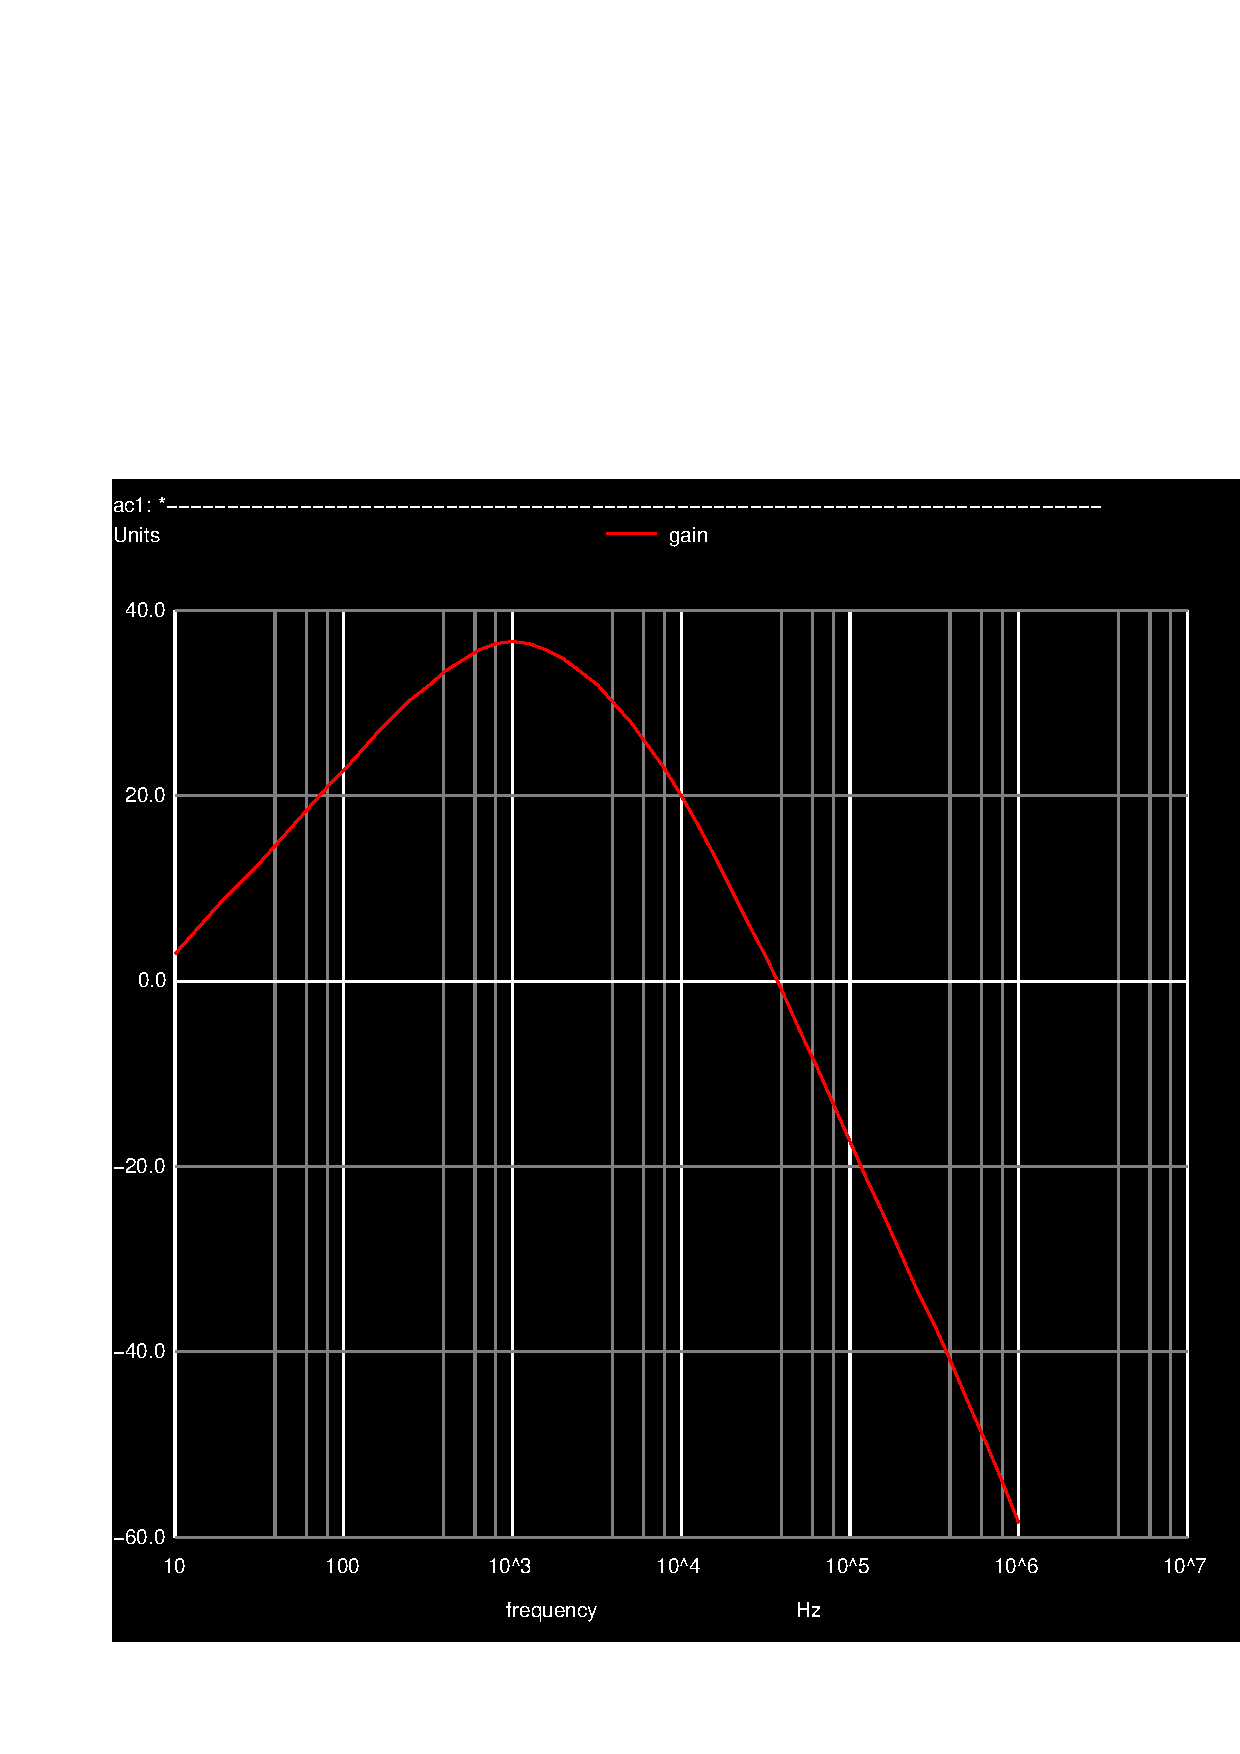
\includegraphics[width = 7cm]{gain.pdf} 
\caption{Gain}
\label{phase}
\end{figure}

\begin{figure}[H] 
\centering
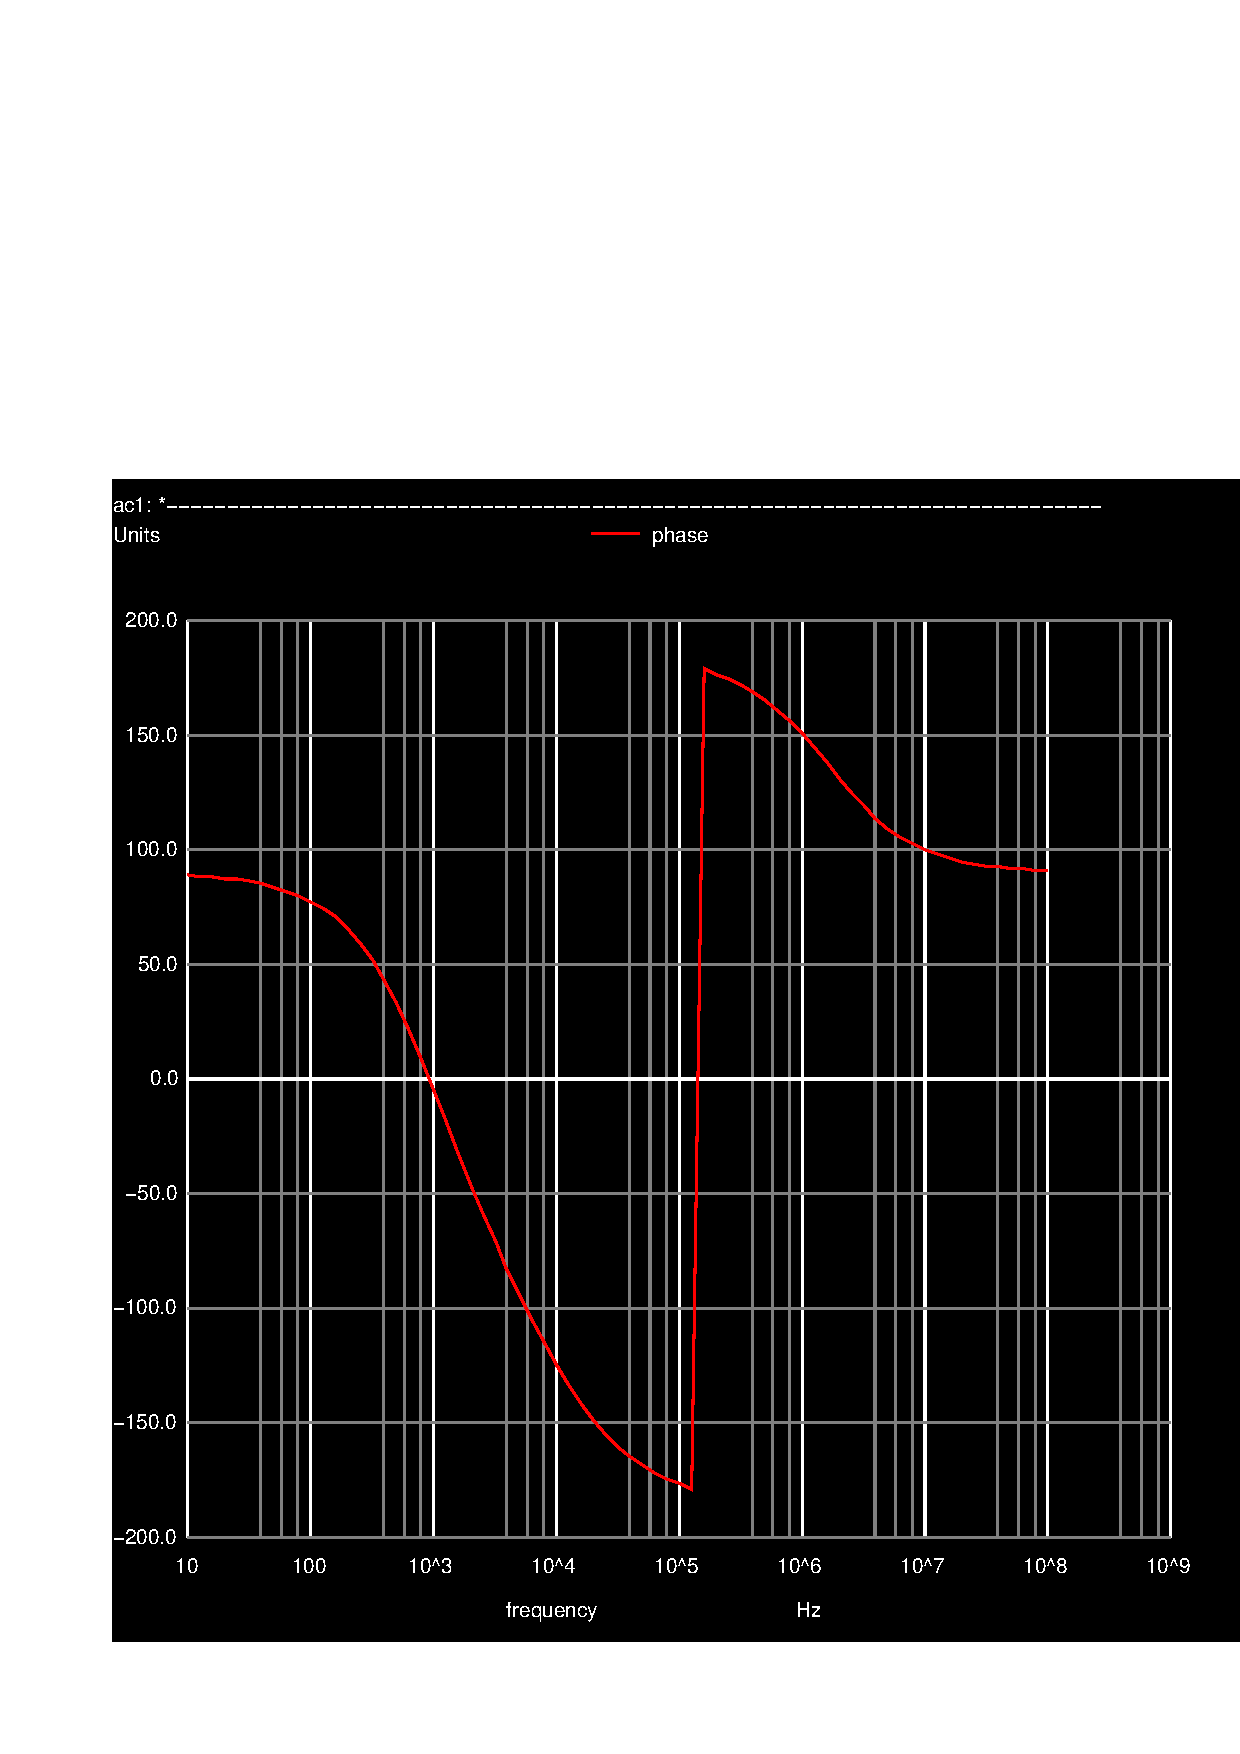
\includegraphics[width = 7cm]{phase.pdf} 
\caption{Phase}
\label{phase}
\end{figure}


\subsection{Input and Output Impedances}

The following table represents the input impedance obtained from simulation in NGSpice:
%Zin
\begin{table}[H] \centering
\begin{tabular}{|
>{\columncolor[HTML]{FFCC67}}l |c|}
\hline
\multicolumn{2}{|l|}{\cellcolor[HTML]{EABD8B}Name - Value} \\ \hline
Zin & -1308.32 + 31.5445 j\\ \hline

\end{tabular}
\caption{Zin}
\end{table}

The result obtained for the input impedance, considering the value in Ohm's, is quite high, wich turns to be very benefitial for the gain, because the voltage in node 2 must be as similiar to Vin as possible. 
Using a voltage divider, the only way to achieve this was to have a very high resistance value.\par

The following table represents the output impedance obtained from simulation in NGSpice:
%Zout
\begin{table}[H] \centering
\begin{tabular}{|
>{\columncolor[HTML]{FFCC67}}l |c|}
\hline
\multicolumn{2}{|l|}{\cellcolor[HTML]{EABD8B}Name - Value} \\ \hline
Zo & 41.2518 + -1.18453 j\\ \hline
Zoarg & 41.2688\\ \hline

\end{tabular}
\caption{Zout}
\end{table}

In regard to the output impedance, an opposite deduction to the one made for the output impedance is needed.  
Using again a voltage divider, the output impedance must be as low as possible, in order to the output voltage to be as high as possible.

\section{Comparison}
\label{comparison}

In this section a global comparison of the two approaches is created, with the chosen values for the constants.  
The following table represents the comparison between the results obtained from Octave and from simulation in NGSpice:
%Results
\begin{table}[H]
    \begin{minipage}{.5\linewidth}
      \centering
        \begin{tabular}{|
		>{\columncolor[HTML]{FFCC67}}l |c|}
		\hline
		\multicolumn{2}{|l|}{\cellcolor[HTML]{EABD8B}Name - Value} \\ \hline
		\input{../mat/results_octave_TAB}
	\end{tabular}
      \caption{Octave}
    \end{minipage}%
    \begin{minipage}{.5\linewidth}
      \centering
        \begin{tabular}{|
		>{\columncolor[HTML]{FFCC67}}l |c|}
		\hline
		\multicolumn{2}{|l|}{\cellcolor[HTML]{EABD8B}Name - Value} \\ \hline
		V-Gain & 63.2292\\ \hline
Bandwidth & 1.33156E+06\\ \hline
CO-lowerFreq & 19.2729\\ \hline
CO-7.5007higherFreq & 1.33158E+06\\ \hline

	\end{tabular}
       \caption{NGspice}
    \end{minipage} 
   \caption{Simulation results - comparison}
\end{table}
%Zin
\begin{table}[H]
    \begin{minipage}{.5\linewidth}
      \centering
        \begin{tabular}{|
		>{\columncolor[HTML]{FFCC67}}l |c|}
		\hline
		\multicolumn{2}{|l|}{\cellcolor[HTML]{EABD8B}Name - Value} \\ \hline
		\input{../mat/zin_TAB}
	\end{tabular}
      \caption{Octave}
    \end{minipage}%
    \begin{minipage}{.5\linewidth}
      \centering
        \begin{tabular}{|
		>{\columncolor[HTML]{FFCC67}}l |c|}
		\hline
		\multicolumn{2}{|l|}{\cellcolor[HTML]{EABD8B}Name - Value} \\ \hline
		Zin & -1308.32 + 31.5445 j\\ \hline

	\end{tabular}
       \caption{NGspice}
    \end{minipage} 
   \caption{Zin comparison}
\end{table}
%Zout
\begin{table}[H]
    \begin{minipage}{.5\linewidth}
      \centering
        \begin{tabular}{|
		>{\columncolor[HTML]{FFCC67}}l |c|}
		\hline
		\multicolumn{2}{|l|}{\cellcolor[HTML]{EABD8B}Name - Value} \\ \hline
		\input{../mat/zout_TAB}
	\end{tabular}
      \caption{Octave}
    \end{minipage}%
    \begin{minipage}{.5\linewidth}
      \centering
        \begin{tabular}{|
		>{\columncolor[HTML]{FFCC67}}l |c|}
		\hline
		\multicolumn{2}{|l|}{\cellcolor[HTML]{EABD8B}Name - Value} \\ \hline
		Zo & 41.2518 + -1.18453 j\\ \hline
Zoarg & 41.2688\\ \hline

	\end{tabular}
       \caption{NGspice}
    \end{minipage} 
   \caption{Zout comparison}
\end{table}

As seen in the previous table, as requested, we were able to compute the passband frequency in a simulation analysis using the measure funtion and the central frequency in the theoretical analysis as explained in Section~\ref{sec:analysis}.  We have to consider that the OP-Amp model chosen is far more complex in Ngspice than in Octave. The different calculation methods lead to the difference between both methods, being that the calculated and simulated impedances have the same issues, explaining why there is a significant variation between impedances of both analyses.

Next we present both theoretical and simulation graphs of the frequency response of the gain and the phase side by side.

%Gain comparison

\begin{figure}[H] 
\centering
\begin{subfigure}{0.4\textwidth}
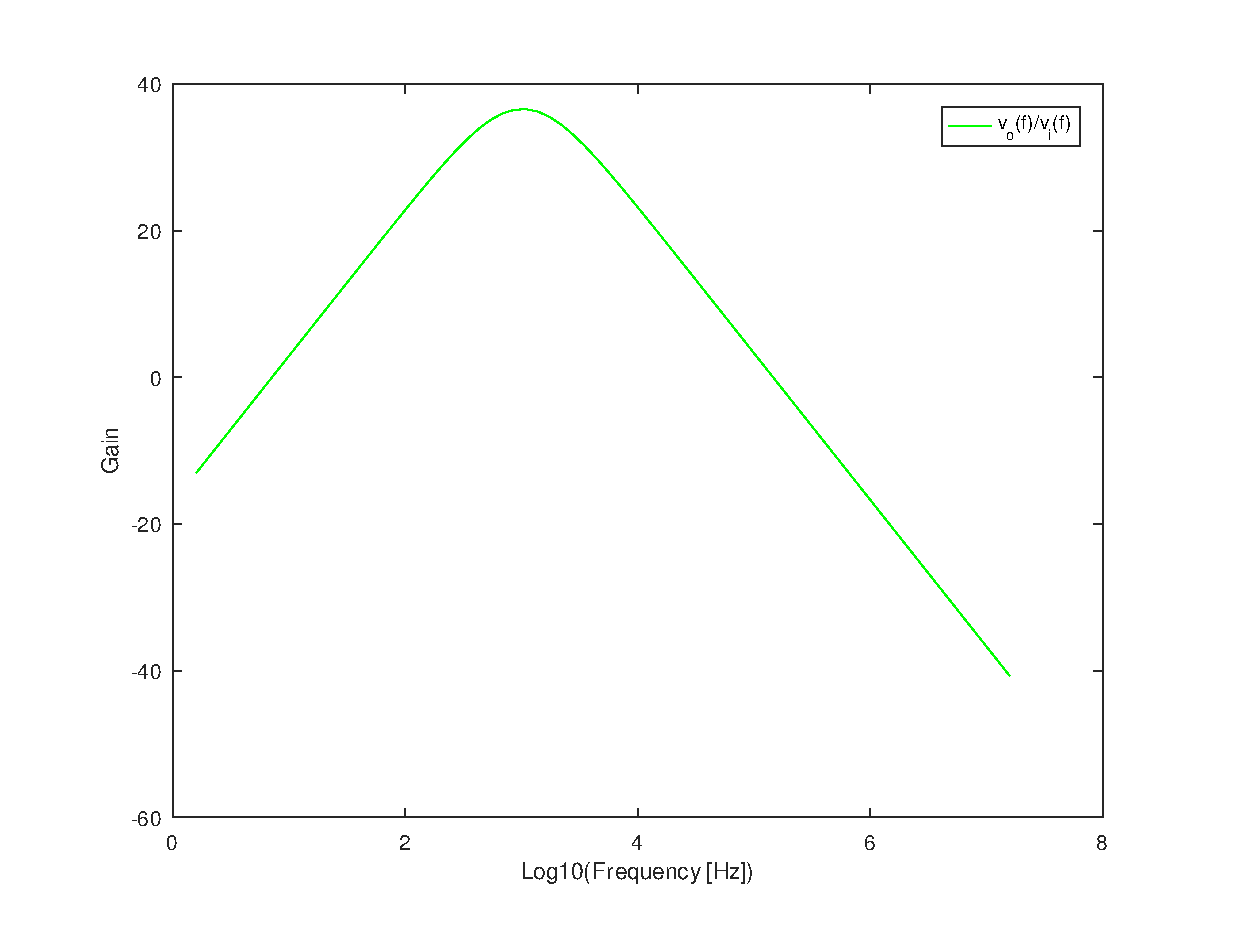
\includegraphics[width=\textwidth]{gain.eps}
\caption{OCTAVE}
\label{Octave_gain}
\end{subfigure}
\begin{subfigure}{0.3\textwidth}
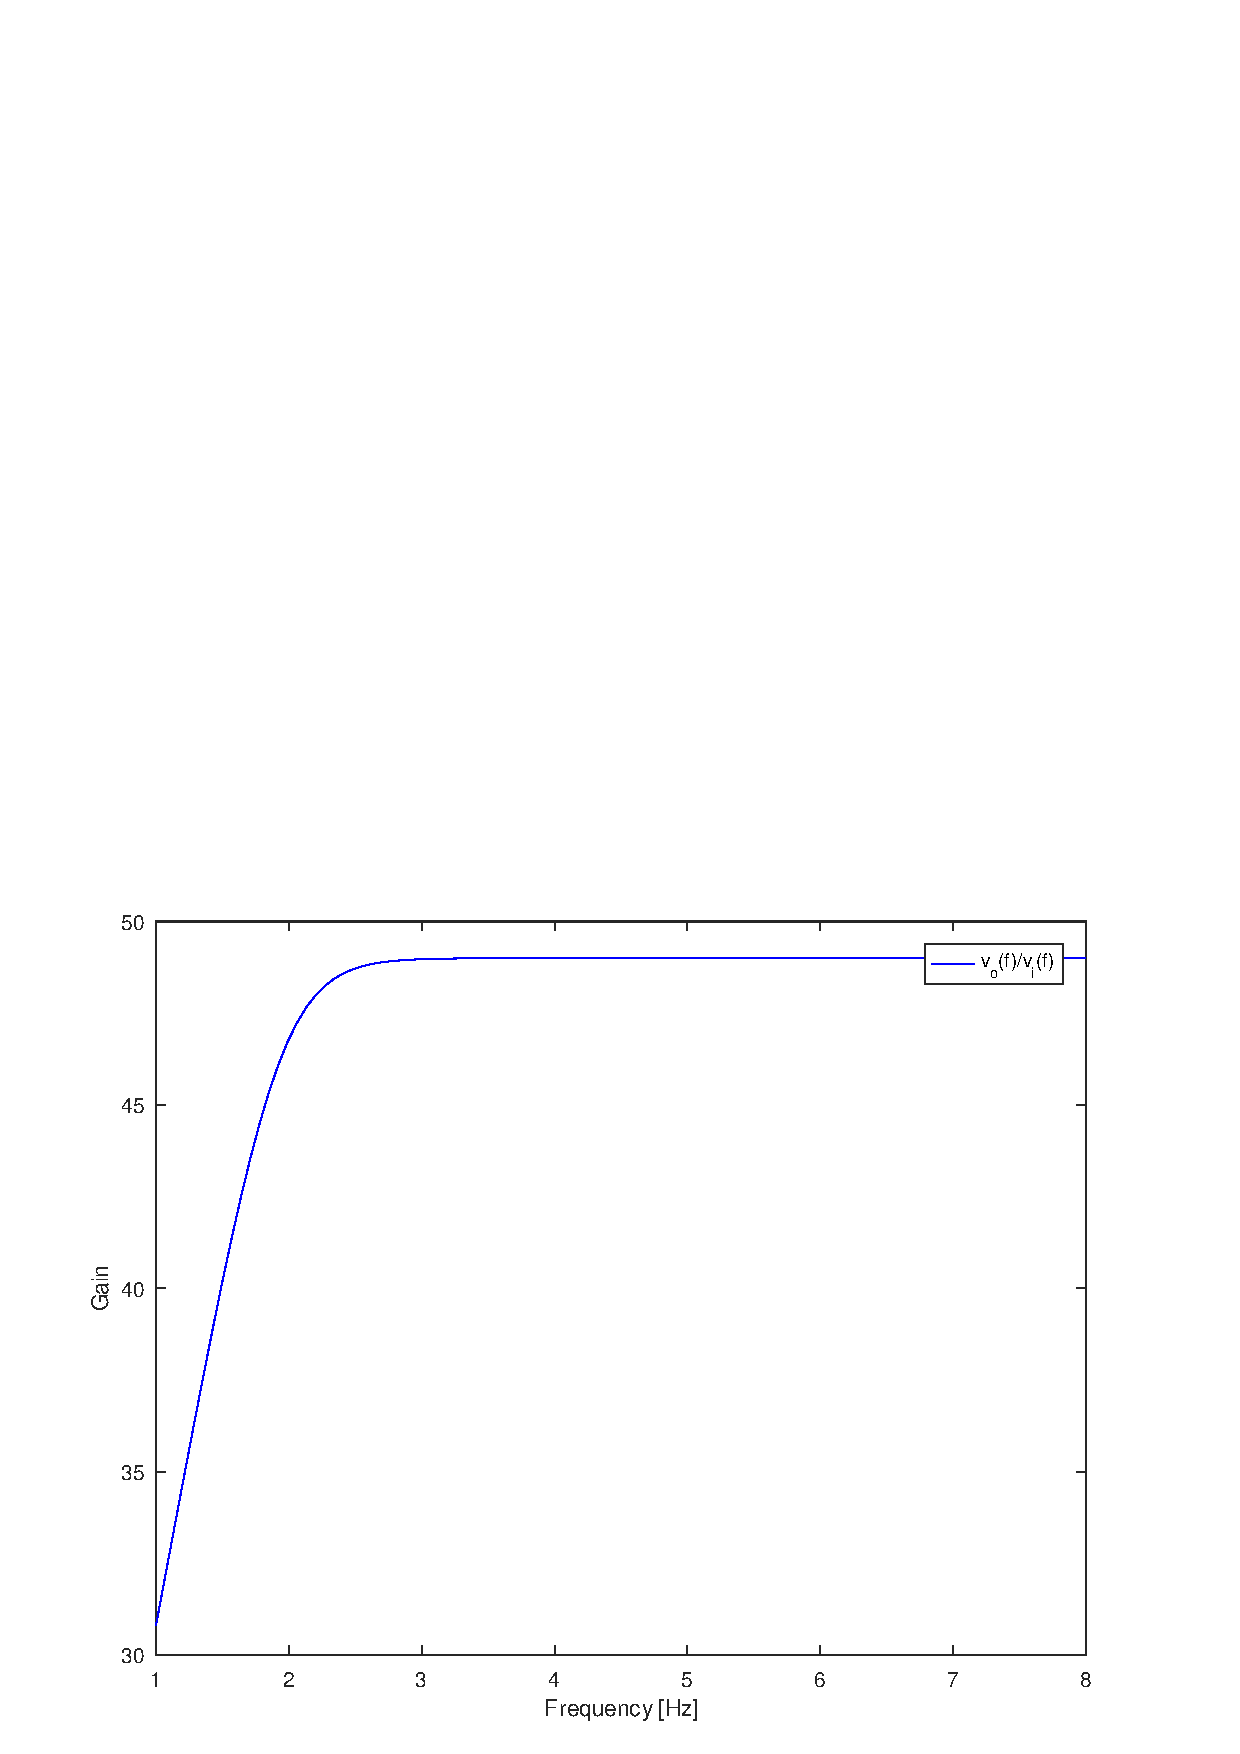
\includegraphics[width=\textwidth]{Gain.pdf}
\caption{NGSPICE}
\label{Ngspice_gain}
\end{subfigure}
\caption{Gain}
\end{figure}

%phase

\begin{figure}[H] 
\centering
\begin{subfigure}{0.4\textwidth}
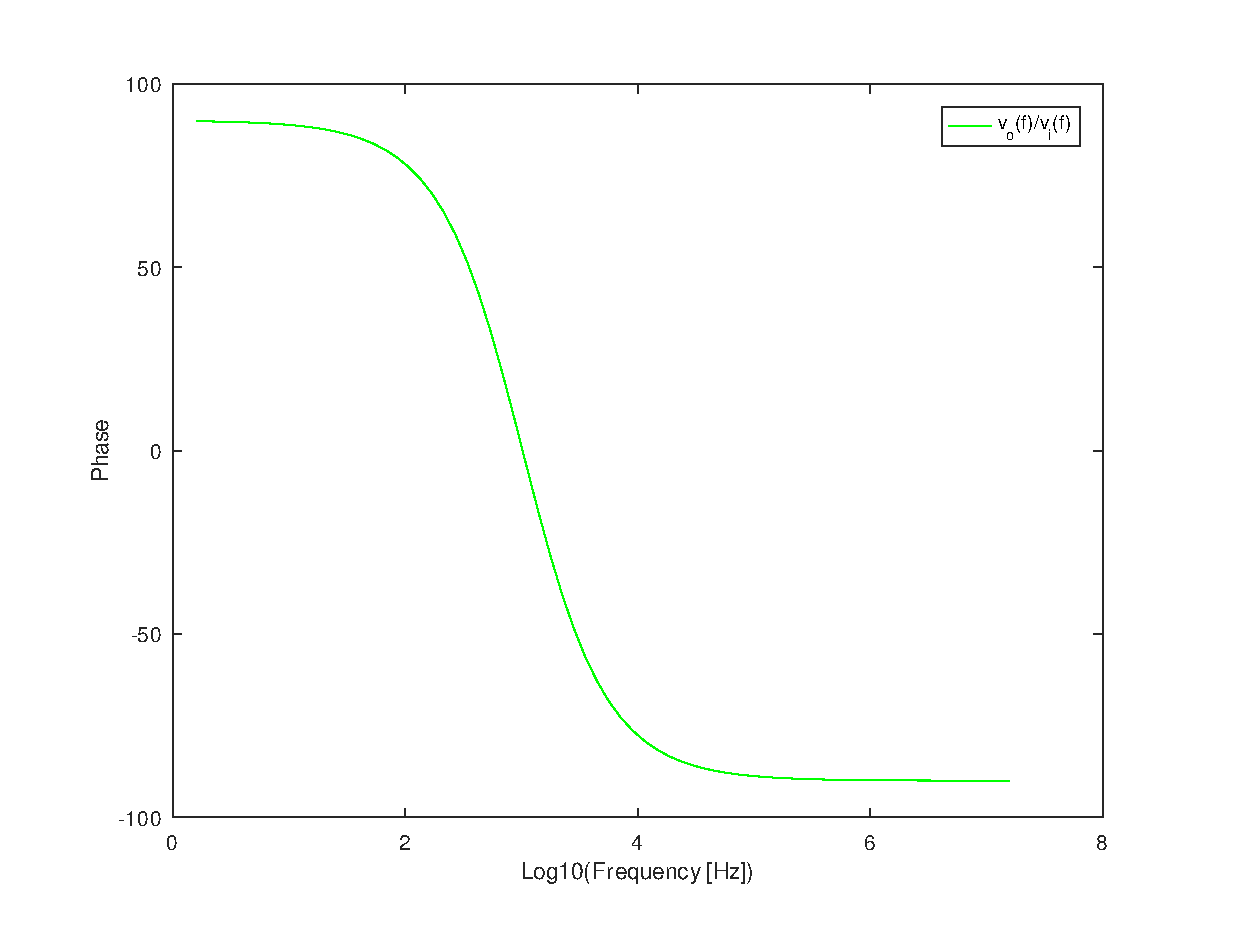
\includegraphics[width=\textwidth]{phase.eps}
\caption{OCTAVE}
\label{Octave_phase}
\end{subfigure}
\begin{subfigure}{0.3\textwidth}
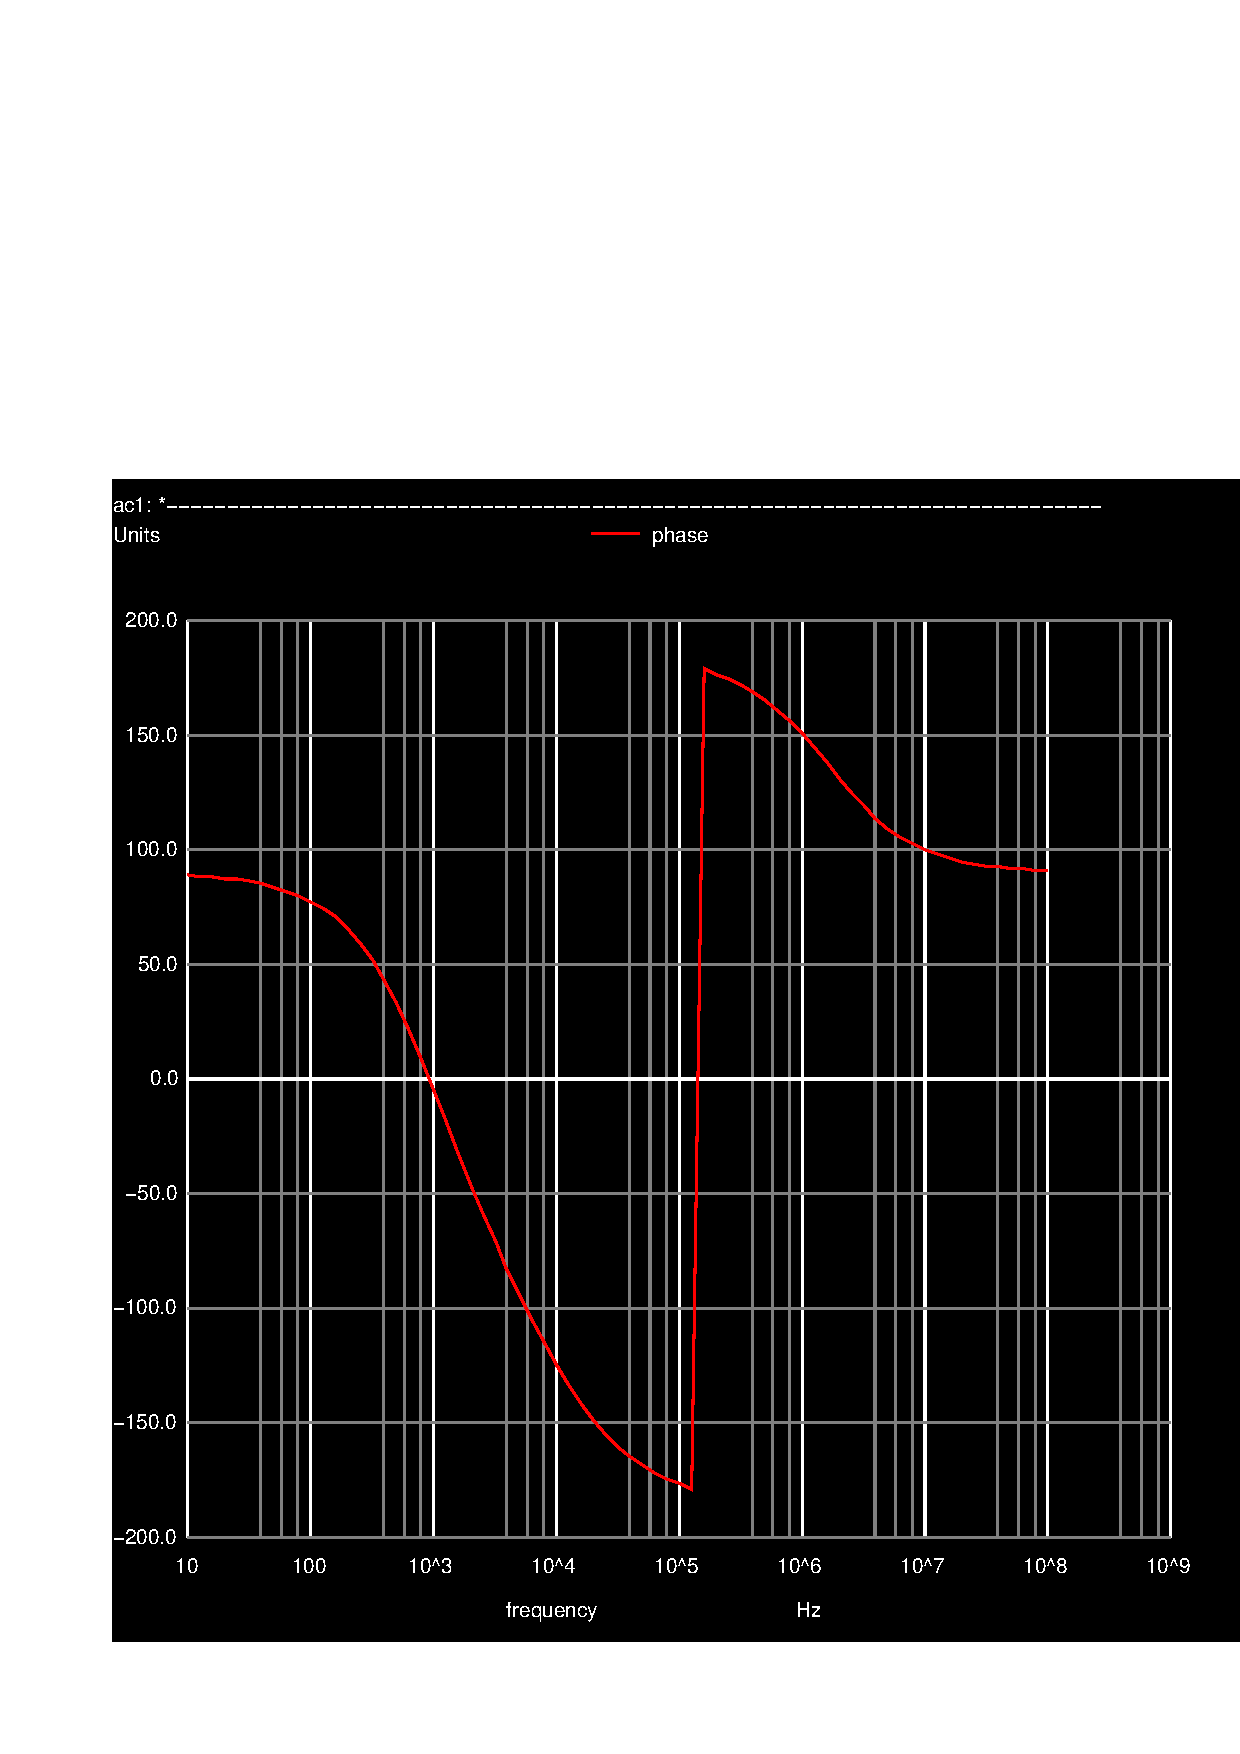
\includegraphics[width=\textwidth]{phase.pdf}
\caption{NGSPICE}
\label{Ngspice_phase}
\end{subfigure}
\caption{Phase}
\end{figure}

In general, in terms of the graphs, we achieved satisfactory results.  When an initial comparison of the gain response is executed, using the shape of the graph, isn't difficult to realise that they have a similar behaviour. As seen in the upper graphs, in the initial section, there is a constant slope of +20dB/dec. After that, exists a small pass band, that is also the region where the central frequency is achieved, and a last part with a slope of -20dB/dec.\par
When it comes to the lower grpahs, in the phase response, both plots differ.  This is because our theoretical model does not predict the existence of capacitors in the OP AMP, as it idealises the gain as being purely real, i.e, there's no shift in phase. In reality, because the OP AMP has two capacitors, it is expected that in the phase frequency response plot each would introduce a shift of -90º,  making the overall phase to go down to -270º, in other words, +90º. As we can observe from the initial table of this Section (~\ref{comparison}) we have small relative errors for the values of interest. This somehow proves that, eventhough the OP AMP's are made of dozens of components, being some of them non-linear, we can predict its behaviour.


\section{Merit Results}
\label{merit}

From the results obtained through the Ngspice simulation and considering we used the data shown in table 1, we can compute the merit using the formula given in the lab assignment, represented in the Introduction.

The values of cost and merit are represented in the next table:

\begin{table}[H]
    \begin{minipage}{.5\linewidth}
      \centering
        \begin{tabular}{|
		>{\columncolor[HTML]{FFCC67}}l |c|}
		\hline
		\multicolumn{2}{|l|}{\cellcolor[HTML]{EABD8B}Name - Value} \\ \hline
		Cost & 2.639850e+02 \\ \hline
Merit & 1.428277e-04 \\ \hline

	\end{tabular}
      \caption{Octave}
    \end{minipage}%
    \begin{minipage}{.5\linewidth}
      \centering
        \begin{tabular}{|
		>{\columncolor[HTML]{FFCC67}}l |c|}
		\hline
		\multicolumn{2}{|l|}{\cellcolor[HTML]{EABD8B}Name - Value} \\ \hline
		Cost & 2619.6\\ \hline
merit & 1262.83\\ \hline

	\end{tabular}
       \caption{NGspice}
    \end{minipage} 
   \caption{Cost and Merit}
\end{table}
